% This is samplepaper.tex, a sample chapter demonstrating the
% LLNCS macro package for Springer Computer Science proceedings;
% Version 2.20 of 2017/10/04
%
\documentclass[runningheads]{llncs}
%
\usepackage{graphicx}

% Used for displaying a sample figure. If possible, figure files should
% be included in EPS format.
%
% If you use the hyperref package, please uncomment the following line
% to display URLs in blue roman font according to Springer's eBook style:
% \renewcommand\UrlFont{\color{blue}\rmfamily}

\begin{document}
\newcommand{\ywa}[1]{\textsf{#1}}

%
\title{Towards More Reproducible Data Wrangling with OpenRefine\thanks{This work was supported by the US National Science Foundation NSF: OAC \#1541450}}
%
%\titlerunning{Abbreviated paper title}
% If the paper title is too long for the running head, you can set
% an abbreviated paper title here
%
% \author{\relax}
\author{Lan Li\inst{1} \and
Qian Zhang\inst{2} \and
Bertram Ludäscher\inst{1}}
%
%\authorrunning{F. Author et al.}
% First names are abbreviated in the running head.
% If there are more than two authors, 'et al.' is used.
%
% \institute{\relax}
\institute{University of Illinois at Urbana-Champaign, Champaign, IL, USA 
\email{\{lanl2,ludaesch\}@illinois.edu}
\and
University of Waterloo, 200 University Ave W, Waterloo ON N2L 3G1, Canada
\email{q394zhan@uwaterloo.ca}\\
}

\maketitle              % typeset the header of the contribution
%
\begin{abstract}
OpenRefine (OR) is a popular data wrangling tool. During data cleaning , not only a processed dataset will be generated but also some other provenance-related byproducts. One of them is a native OR recipe (JSON file), and the other one is the Operation History (OH) that lists a series of human-readable data cleaning steps, both of which promote research transparency to some extent by containing some (but incomplete) prospective provenance and partial retrospective provenance information~\cite{ref_proc1}, making them difficult to be directly used for reuse and Reproducibility from OpenRefine Web API (see Fig.~\ref{fig1}). In this poster, a prototype consisting of two sub-systems, one of which extends the native OR recipe to generate a complete recipe (a.k.a. enhanced receipt)  followed by the second re-runner system, is created to complement the missing information between the actual data cleaning operations and the native OR recipe, which meanwhile facilitates transparency, reproducibility and reusability. 

\keywords{OpenRefine \and transparency \and reproducibility \and reusability}
\end{abstract}

\begin{figure}
\centering
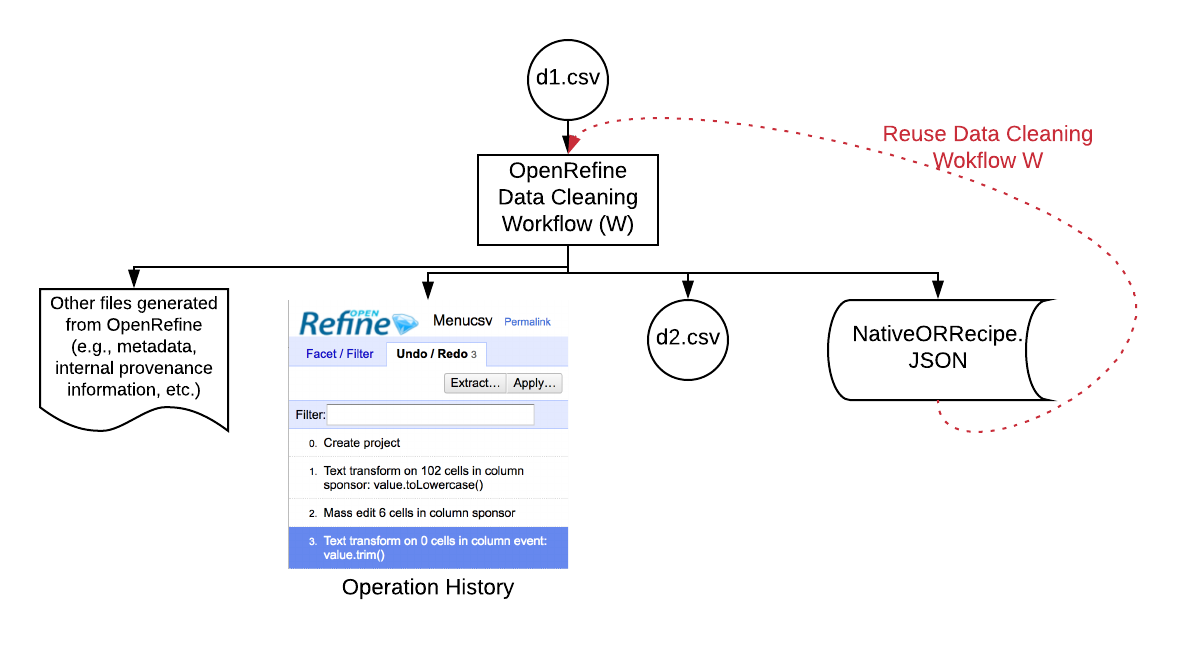
\includegraphics[width=100mm,scale=0.7]{figs/DC.png}
\caption{Data Wrangling in OpenRefine} \label{fig1}
\end{figure}



%
%
%
\section{Introduction}
OpenRefine is used for data wrangling and data cleaning in many areas nowadays. Data cleaning can be understood as taking (presumably "messy") input data $d1.csv$, subjecting it to a data cleaning procedure or workflow $W$, resulting in an (presumably "clean(er)") output data $d2.csv$\footnote[1]{The desiderata for $d2.csv$ include that it is a “better” or more accurate model of reality than $d1.csv$, and that $d2.csv$ is “fit for use/purpose” (whereas $d2.csv$ might not have been). But this is not our concern here.} (see Fig.~\ref{fig1}). When presenting $d2.csv$ three properties are often considered important: a). \textbf{Transparency}: Being transparent about what happened to $d1.csv$ to obtain $d2.csv$. For example, to document “everything” that happened, in particular make sure $W$'0s operations (and parameters) are clearly documented, which is primarily about retrospective provenance~\cite{ref_lncs1}. b). \textbf{Reproducibility}: Being closely related to transparency. The focus lies in that a user should be able to take the workflow $W$ (possibly re-implemented in another language ⇒ $W’$), apply it to $d1.csv$ and obtain the same result, i.e., let \(d3=W'(P,d1)\), where $P$ are any additional inputs (in particular parameters) that are needed to re-execute $W$ on $d1$ to make sure we obtain the same\footnote[1]{In more general settings “same” could be relaxed to “equivalent”. Here, for simplicity, by “same” we mean the same bit-level representation (in practice: a “diff“ between $d2$ and $d1$ will show no differences).} output $d2$. Then \(d3=d2\).
 And c). \textbf{Reusability}: The data cleaning workflow $W$ developed originally for $d1$ should be readily applicable to “similar“ dataset $e1.csv$. That is, we want to reuse $W$ on $e1.csv$ and become a meaningfully “better“ dataset \(e2 = W(e1)\). The strength of OpenRefine lies in that it has already supported transparency, reproducibility and reusability to some extent, in a way that the operation history (a.k.a. recipe) provides a JSON representation (a.k.a. native OR recipe) of most of the operation that OR has performed on a given dataset/project. However, after studying OR recipes and other "sideways/internal provenance information" of OR, we found the following shortcomings: First of all, the native OR recipe shows limited transparency. For example, when the user performs some common transformations such as \ywa{\emph{To lowercase}}  operation, native OR recipe only captures the operation name \textbf{without} recording the actual change of the records (i.e., \ywa{"from": [...]}, \ywa{"to": ...}). The other extreme example is the "single-cell edit" operation, for which neither the operation name nor the operation effect is recorded at all in the native OR recipe (see Fig.~\ref{fig2}). This also demonstrates OR's limited reproducibility issue. Another problem with the native OR recipe is its limited reusability. For example, when the \ywa{\emph{Cluster and edit}} operation is performed, OR captures only the actual change of each record \textbf{without} the underlying “cluster“ method details such as the cluster type, function and/or associated parameter settings. In this way, this native OR recipe can not be reused with the updated dataset.


\begin{figure}
\centering
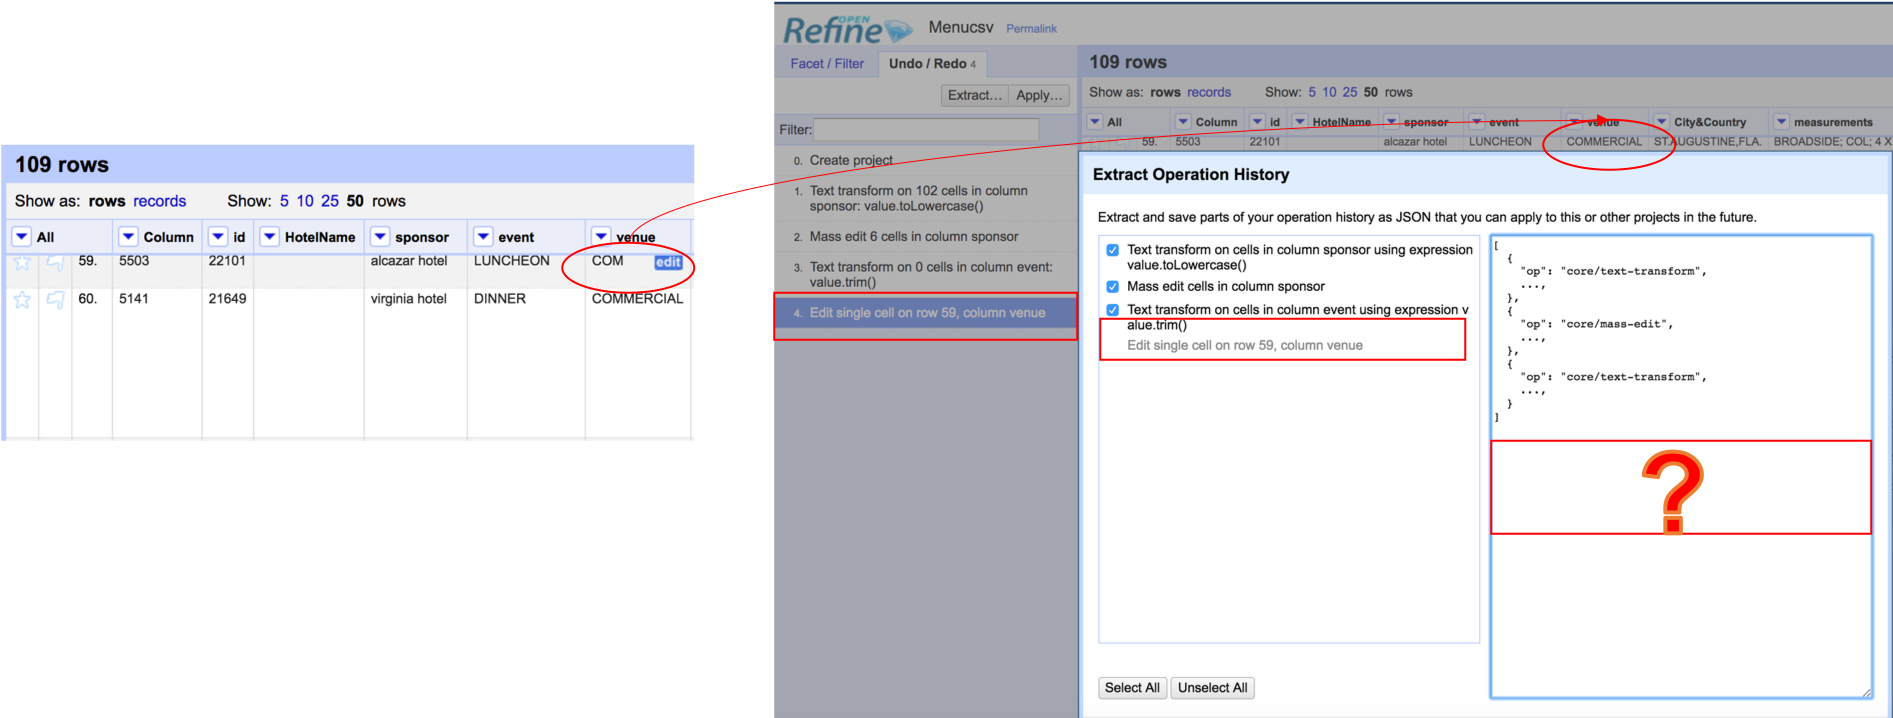
\includegraphics[width=100mm]{figs/singleedit.png}\
\caption{Missing Info with Single Cell Edit Operation} \label{fig2}
\end{figure}


\section{Contributions}
In this poster, a CLI (command line interface) prototype consisting of two sub-systems is developed by extending the OpenRefine Python Client Library (OR-client)~\cite{ref_url1}. The first one is named CLOPER (Command-Line OpenRefine Prototype for Enhanced Recipe), which makes the incomplete native OR recipe complete to improve OR's transparency and reusability. And the ERRR system (Enhanced Recipe Re-Runner) verifies the resproducility of the enhanced recipe derived from CLOPER.

\section{Prototype}
The prototype includes two sub-systems. 
\subsection{Command-Line OpenRefine Prototype for Enhanced Recipe} CLOPER (see Fig.~\ref{fig3}) aims to enhance transparency and reusability of the native OR recipe, which reads in the original "messy" dataset ($d1.csv$) and communicates with an OR server through the interface provided by the OR-client. The outputs consist of three products: an enhanced recipe ($EnhancedRecipe.JSON$) is generated at the back-end; a "cleaned" dataet ($d2.csv$) and a native OR recipe ($NativeORRecipe.JSON$) are exported from the OR web UI. 
\subsection{Enhanced Recipe Re-Runner}
In regards to reproducibility, ERRR (see Fig.~\ref{fig4}) re-implements the enhanced recipe ($EnhancedRecipe.JSON$) that is derived from CLOPER, applies to the same original "messy" dataset ($d1.csv$). Again ERRR connects to an OR server via OR-client and obtains the same output ($d2.csv$) associated with the native OR recipe ($NativeORRecipe.JSON$).

A subset of the OR operations (e.g., \ywa{\emph{Cluster and edit}}, \ywa{\emph{To lowercase}}, \ywa{\emph{To date}} , etc.) were used to test both sub-systems of the proposed prototype. The results showed that the enhanced OR recipe improved the transparency, reproducibility and reusability compared to the native OR recipe. 

\begin{figure}
    \centering
    \begin{minipage}{0.55\textwidth}
        \centering
        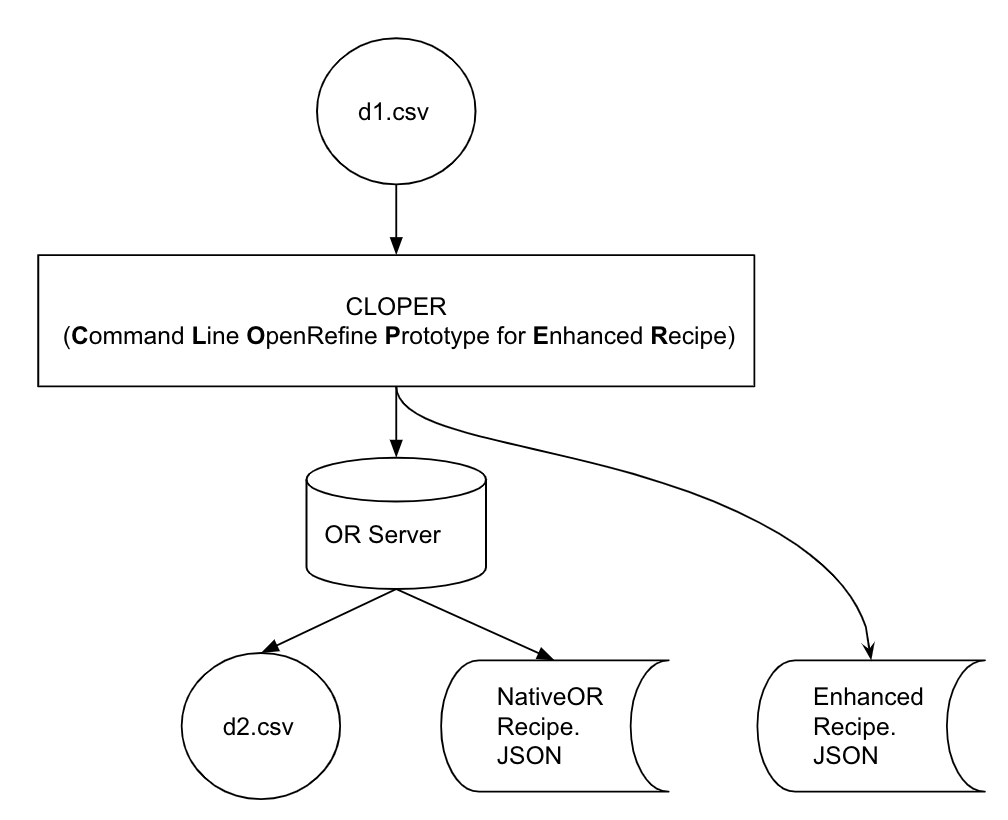
\includegraphics[width=0.9\textwidth]{figs/CLOPER.png} % first figure itself
        \caption{Command Line OpenRefine Prototype for Enhanced Recipe(CLOPER)}\label{fig3}\centering
    \end{minipage}\hfill
    \begin{minipage}{0.4\textwidth}
        \centering
        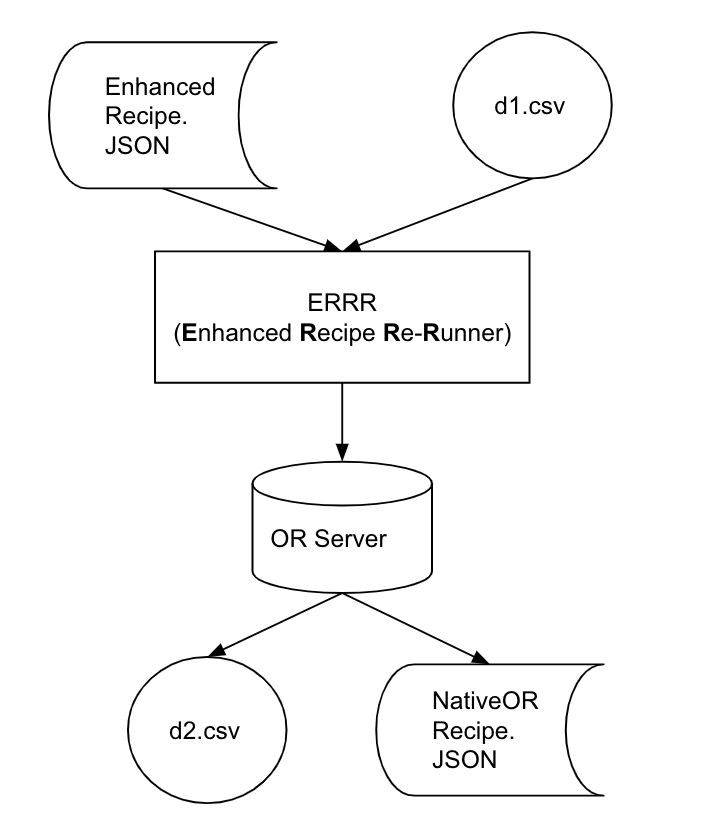
\includegraphics[width=0.9\textwidth]{figs/ERRR.png} % second figure itself
        \caption{Enhanced Recipe Re-Runner(ERRR)}\label{fig4}\centering
    \end{minipage}
\end{figure}

\section{Further Work}
For the further work, more operations (e.g.,\ywa{\emph{single-cell edit}}) need to be improved by fixing the incomplete and/or missing information (see Fig.~\ref{fig2}). In order to advance reproducibility of the enhanced recipe, CLOPER is expected to assist in capturing more prospective and retrospective provenance. 

\begin{thebibliography}{8}

\bibitem{ref_proc1}
Dey, S., Belhajjame, K., Koop, D., Raul, M.,Ludscher, B.:Linking prospective and retrospective provenance in scripts. In: Theory and Practice of Provenance. In: 9 International Journal of Digital Curation. (2015)

\bibitem{ref_lncs1}
Zhao, Y., Wilde, M., Foster, I.:Applying the virtual data provenance model. In: International Provenance and Annotation Workshop pp. 148-161. Springer, Berlin, Heidelberg.(2006, May)

\bibitem{ref_url1}
OpenRefine-client Library Github, \url{https://github.com/opencultureconsulting/openrefine-client}. 


\end{thebibliography}





\end{document}

